\documentclass[12pt,a4paper]{article}

\usepackage[a4paper,margin=1in]{geometry}
\usepackage{graphicx}
\usepackage{booktabs}
\usepackage{amsmath,amssymb}
\usepackage{float}
\usepackage{hyperref}
\usepackage{xcolor}
\usepackage{listings}
\usepackage{enumitem}
\usepackage{fancyhdr}
\usepackage{longtable}

\hypersetup{colorlinks=true,linkcolor=blue,urlcolor=blue}

\pagestyle{fancy}
\fancyhf{}
\lhead{ICS1512}
\rhead{Machine Learning Laboratory}
\cfoot{\thepage}

\begin{document}

\begin{tabular}{|p{4cm}|p{11.5cm}|}
\hline
Experiment No. & 7 \\ \hline
Experiment Title & Bagging, Boosting, and Stacked Ensemble Models \\ \hline
Student Name & \\ \hline
Register Number & \\ \hline
Faculty & Dr. Poreddy Ajay Kumar Reddy \\ \hline
Submission Date & \\ \hline
\end{tabular}

\vspace{0.5cm}

\section{Aim and Objective}
The primary objectives of this experiment are:
\begin{enumerate}[label=\alph*)]
\item To understand ensemble learning strategies: Bagging (Bootstrap Aggregation), Boosting (AdaBoost and Gradient Boosting), and Stacking (Meta-Learning).
\item To implement Bagging and Boosting classifiers on a clinical diagnostic dataset.
\item To build a Stacked Ensemble model combining diverse heterogeneous base learners with a meta-classifier.
\item To compare ensemble models in terms of classification accuracy, precision, recall, F1-score, and generalization stability.
\item To analyze the empirical effect of ensemble methods on the bias--variance trade-off.
\end{enumerate}

\section{Dataset Details, EDA, and Preprocessing Steps}
The experiment is conducted on the \textbf{Wisconsin Diagnostic Breast Cancer (WDBC)} dataset from the UCI Machine Learning Repository.

\begin{table}[H]
\centering
\caption{Dataset Profile and Experimental Setup}
\label{tab:dataset_specs}
\begin{tabular}{|p{6cm}|p{9cm}|}
\hline
\textbf{Dataset Attribute} & \textbf{Specification} \\ \hline
Total Samples & 569 instances \\ \hline
Features & 30 real-valued numerical attributes \\ \hline
Target Classes & Malignant ($M$, $y=0$, 212 samples, 37.26\%) \newline Benign ($B$, $y=1$, 357 samples, 62.74\%) \\ \hline
Missing Values & None (0 missing values present) \\ \hline
Dataset Source Link & \url{https://archive.ics.uci.edu} \\ \hline
Train--Test Partition & 80\% Training ($N=455$), 20\% Testing ($N=114$), Stratified \\ \hline
Feature Standardization & Z-score Normalization (\texttt{StandardScaler}) \\ \hline
Validation Protocol & Stratified 5-Fold Cross-Validation on Training Set \\ \hline
\end{tabular}
\end{table}

\subsection{Exploratory Data Analysis (EDA)}
Exploratory analysis reveals that the 30 continuous features measure three mathematical summaries (mean, standard error, and "worst"/largest value) for 10 distinct morphological properties of cell nuclei: radius, texture, perimeter, area, smoothness, compactness, concavity, concave points, symmetry, and fractal dimension. 
High pairwise correlation ($\rho > 0.95$) exists between geometric size metrics (mean perimeter, mean radius, and mean area). The dataset exhibits a mild class imbalance ($37.3\%$ Malignant vs. $62.7\%$ Benign), which is addressed by utilizing Stratified K-Fold partitioning and evaluating harmonic F1-score alongside ROC-AUC.

\subsection{Preprocessing and Leakage Prevention}
All 30 continuous features are standardized to zero mean and unit variance using \texttt{StandardScaler}:
\begin{equation}
z_j = \frac{x_j - \mu_j}{\sigma_j}
\end{equation}
Scalers are fitted strictly on training folds to prevent data leakage into validation or test folds.

\section{Ensemble Models and Implementation}

\subsection{Bagging (Bootstrap Aggregation)}
Bagging trains $B$ independent base estimators $h_1(x), \dots, h_B(x)$ in parallel on bootstrap samples drawn uniformly with replacement from the training set. Predictions are aggregated via majority voting:
\begin{equation}
\hat{H}_{\text{bag}}(x) = \text{sign}\left(\frac{1}{B}\sum_{b=1}^B h_b(x)\right)
\end{equation}
\begin{itemize}
\item \textbf{Base Estimator:} Unpruned Decision Tree (\texttt{DecisionTreeClassifier}).
\item \textbf{Mechanism:} Eliminates high variance inherent in deep decision trees without inflating bias.
\end{itemize}

\subsection{Boosting: AdaBoost and Gradient Boosting}
Boosting trains models sequentially, where each successive learner focuses on correcting the errors of preceding models:
\begin{itemize}
\item \textbf{AdaBoost:} Dynamically increases sample weights $w_i$ for misclassified samples after each decision stump, concentrating subsequent weak learners on difficult boundary instances.
\item \textbf{Gradient Boosting:} Fits successive regression trees directly to the negative gradients (pseudo-residuals) of the cross-entropy deviance loss:
\begin{equation}
r_{im} = -\left[\frac{\partial L(y_i, F(x_i))}{\partial F(x_i)}\right]_{F=F_{m-1}} = y_i - p_i
\end{equation}
Shrinkage learning rate $\eta \in (0, 1]$ scales each step, systematically driving model bias toward zero.
\end{itemize}

\subsection{Stacked Ensemble (Stacking)}
Stacking combines heterogeneous models drawn from distinct algorithmic families:
\begin{itemize}
\item \textbf{Base Models:} Support Vector Classifier (RBF kernel), Gaussian Na\"\i ve Bayes, and Decision Tree.
\item \textbf{Meta-Learner:} Logistic Regression.
\item \textbf{Implementation:} To eliminate target leakage, 5-fold cross-validated out-of-fold probability predictions $\hat{\mathbf{z}}_i$ are generated during training and supplied as input features to the meta-classifier:
\begin{equation}
\hat{y} = \sigma\left(\mathbf{w}^T \hat{\mathbf{z}} + b\right)
\end{equation}
\end{itemize}

\section{Hyperparameter Exploration and Evaluation Results}
Hyperparameters were evaluated across all ensemble architectures using Stratified 5-Fold Cross-Validation on the training partition.

\subsection{Bagging Results}
Table \ref{tab:bagging} presents the cross-validation performance across ensemble sizes ($n\_estimators$), sample fractions ($max\_samples$), and feature fractions ($max\_features$).

\begin{table}[H]
\centering
\caption{Table 1: Bagging Hyperparameter Evaluation (Base Estimator: Decision Tree)}
\label{tab:bagging}
\begin{tabular}{|c|c|c|c|c|}
\hline
\textbf{$n\_estimators$} & \textbf{$max\_samples$} & \textbf{$max\_features$} & \textbf{Avg CV Accuracy (\%)} & \textbf{Avg CV F1 Score} \\ \hline
10 & 0.5 & 1.0 & 94.51\% & 0.9556 \\ \hline
10 & 0.7 & 1.0 & 95.16\% & 0.9611 \\ \hline
10 & 1.0 & 1.0 & 94.95\% & 0.9591 \\ \hline
25 & 0.5 & 1.0 & 94.51\% & 0.9555 \\ \hline
25 & 0.7 & 1.0 & 95.38\% & 0.9631 \\ \hline
25 & 1.0 & 1.0 & 94.95\% & 0.9591 \\ \hline
50 & 0.5 & 1.0 & 94.51\% & 0.9554 \\ \hline
50 & 0.7 & 1.0 & 95.38\% & 0.9631 \\ \hline
50 & 1.0 & 1.0 & 95.16\% & 0.9611 \\ \hline
100 & 0.5 & 1.0 & 94.95\% & 0.9591 \\ \hline
\textbf{100} & \textbf{0.7} & \textbf{1.0} & \textbf{95.82\%} & \textbf{0.9665} \\ \hline
100 & 1.0 & 1.0 & 95.16\% & 0.9609 \\ \hline
\end{tabular}
\end{table}

\subsection{Boosting Results}
Table \ref{tab:boosting} details the evaluation of AdaBoost and Gradient Boosting across tree depths, learning rates, and estimator counts.

\begin{table}[H]
\centering
\caption{Table 2: Boosting Hyperparameter Evaluation (AdaBoost \& Gradient Boosting)}
\label{tab:boosting}
\begin{tabular}{|l|c|c|c|c|c|}
\hline
\textbf{Algorithm} & \textbf{$n\_estimators$} & \textbf{$learning\_rate$} & \textbf{$max\_depth$} & \textbf{Avg CV Acc (\%)} & \textbf{Avg CV F1} \\ \hline
AdaBoost & 25 & 0.05 & 1 (Stump) & 93.19\% & 0.9462 \\ \hline
AdaBoost & 50 & 0.10 & 1 (Stump) & 95.38\% & 0.9633 \\ \hline
AdaBoost & 100 & 0.50 & 1 (Stump) & 97.36\% & 0.9792 \\ \hline
\textbf{AdaBoost} & \textbf{100} & \textbf{1.00} & \textbf{1 (Stump)} & \textbf{98.02\%} & \textbf{0.9844} \\ \hline
Gradient Boosting & 50 & 0.05 & 3 & 94.95\% & 0.9598 \\ \hline
Gradient Boosting & 100 & 0.10 & 3 & 95.16\% & 0.9614 \\ \hline
Gradient Boosting & 150 & 0.10 & 3 & 95.82\% & 0.9669 \\ \hline
\textbf{Gradient Boosting} & \textbf{150} & \textbf{0.20} & \textbf{3} & \textbf{96.48\%} & \textbf{0.9720} \\ \hline
\end{tabular}
\end{table}

\subsection{Stacked Ensemble Results}
Table \ref{tab:stacking} summarizes the 5-fold cross-validation performance across base model combinations combined via Logistic Regression.

\begin{table}[H]
\centering
\caption{Table 3: Stacked Ensemble Evaluation}
\label{tab:stacking}
\begin{tabular}{|p{7.5cm}|p{3.5cm}|c|c|}
\hline
\textbf{Base Models} & \textbf{Meta Learner} & \textbf{Avg CV Acc (\%)} & \textbf{Avg CV F1} \\ \hline
SVM (RBF) + Na\"\i ve Bayes & Logistic Regression & 96.48\% & 0.9718 \\ \hline
Decision Tree + SVM (RBF) & Logistic Regression & 97.14\% & 0.9771 \\ \hline
\textbf{SVM (RBF) + Na\"\i ve Bayes + Decision Tree} & \textbf{Logistic Regression} & \textbf{96.70\%} & \textbf{0.9735} \\ \hline
SVM (RBF) + Na\"\i ve Bayes + Random Forest & Logistic Regression & 96.92\% & 0.9752 \\ \hline
\end{tabular}
\end{table}

\section{Performance Comparison and Evaluation Metrics}
All models were tested on the independent 20\% holdout test set ($N=114$). Table \ref{tab:comparison} reports the evaluation metrics: Accuracy, Precision, Recall, F1-Score, and ROC-AUC.

\begin{table}[H]
\centering
\caption{Table 4: Performance Comparison of Ensemble Models on Holdout Test Set}
\label{tab:comparison}
\begin{tabular}{|l|c|c|c|c|c|}
\hline
\textbf{Model} & \textbf{Accuracy (\%)} & \textbf{Precision} & \textbf{Recall} & \textbf{F1 Score} & \textbf{ROC-AUC} \\ \hline
Single Decision Tree (Baseline) & 91.23\% & 0.9559 & 0.9028 & 0.9286 & 0.9157 \\ \hline
Bagging ($B=100, \text{samples}=0.7$) & 94.74\% & 0.9583 & 0.9583 & 0.9583 & 0.9859 \\ \hline
Boosting: AdaBoost ($B=100, \eta=1.0$) & 95.61\% & 0.9467 & 0.9861 & 0.9660 & 0.9934 \\ \hline
Boosting: Gradient Boosting ($B=150, \eta=0.2$) & 95.61\% & 0.9467 & 0.9861 & 0.9660 & 0.9912 \\ \hline
\textbf{Stacked Ensemble (SVM+NB+DT $\to$ LR)} & \textbf{97.37\%} & \textbf{0.9726} & \textbf{0.9861} & \textbf{0.9793} & \textbf{0.9967} \\ \hline
\end{tabular}
\end{table}

\section{Graphs and Visualizations}
The experimental results are illustrated across Figures \ref{fig:bagging} to \ref{fig:feat}.

\begin{figure}[H]
\centering
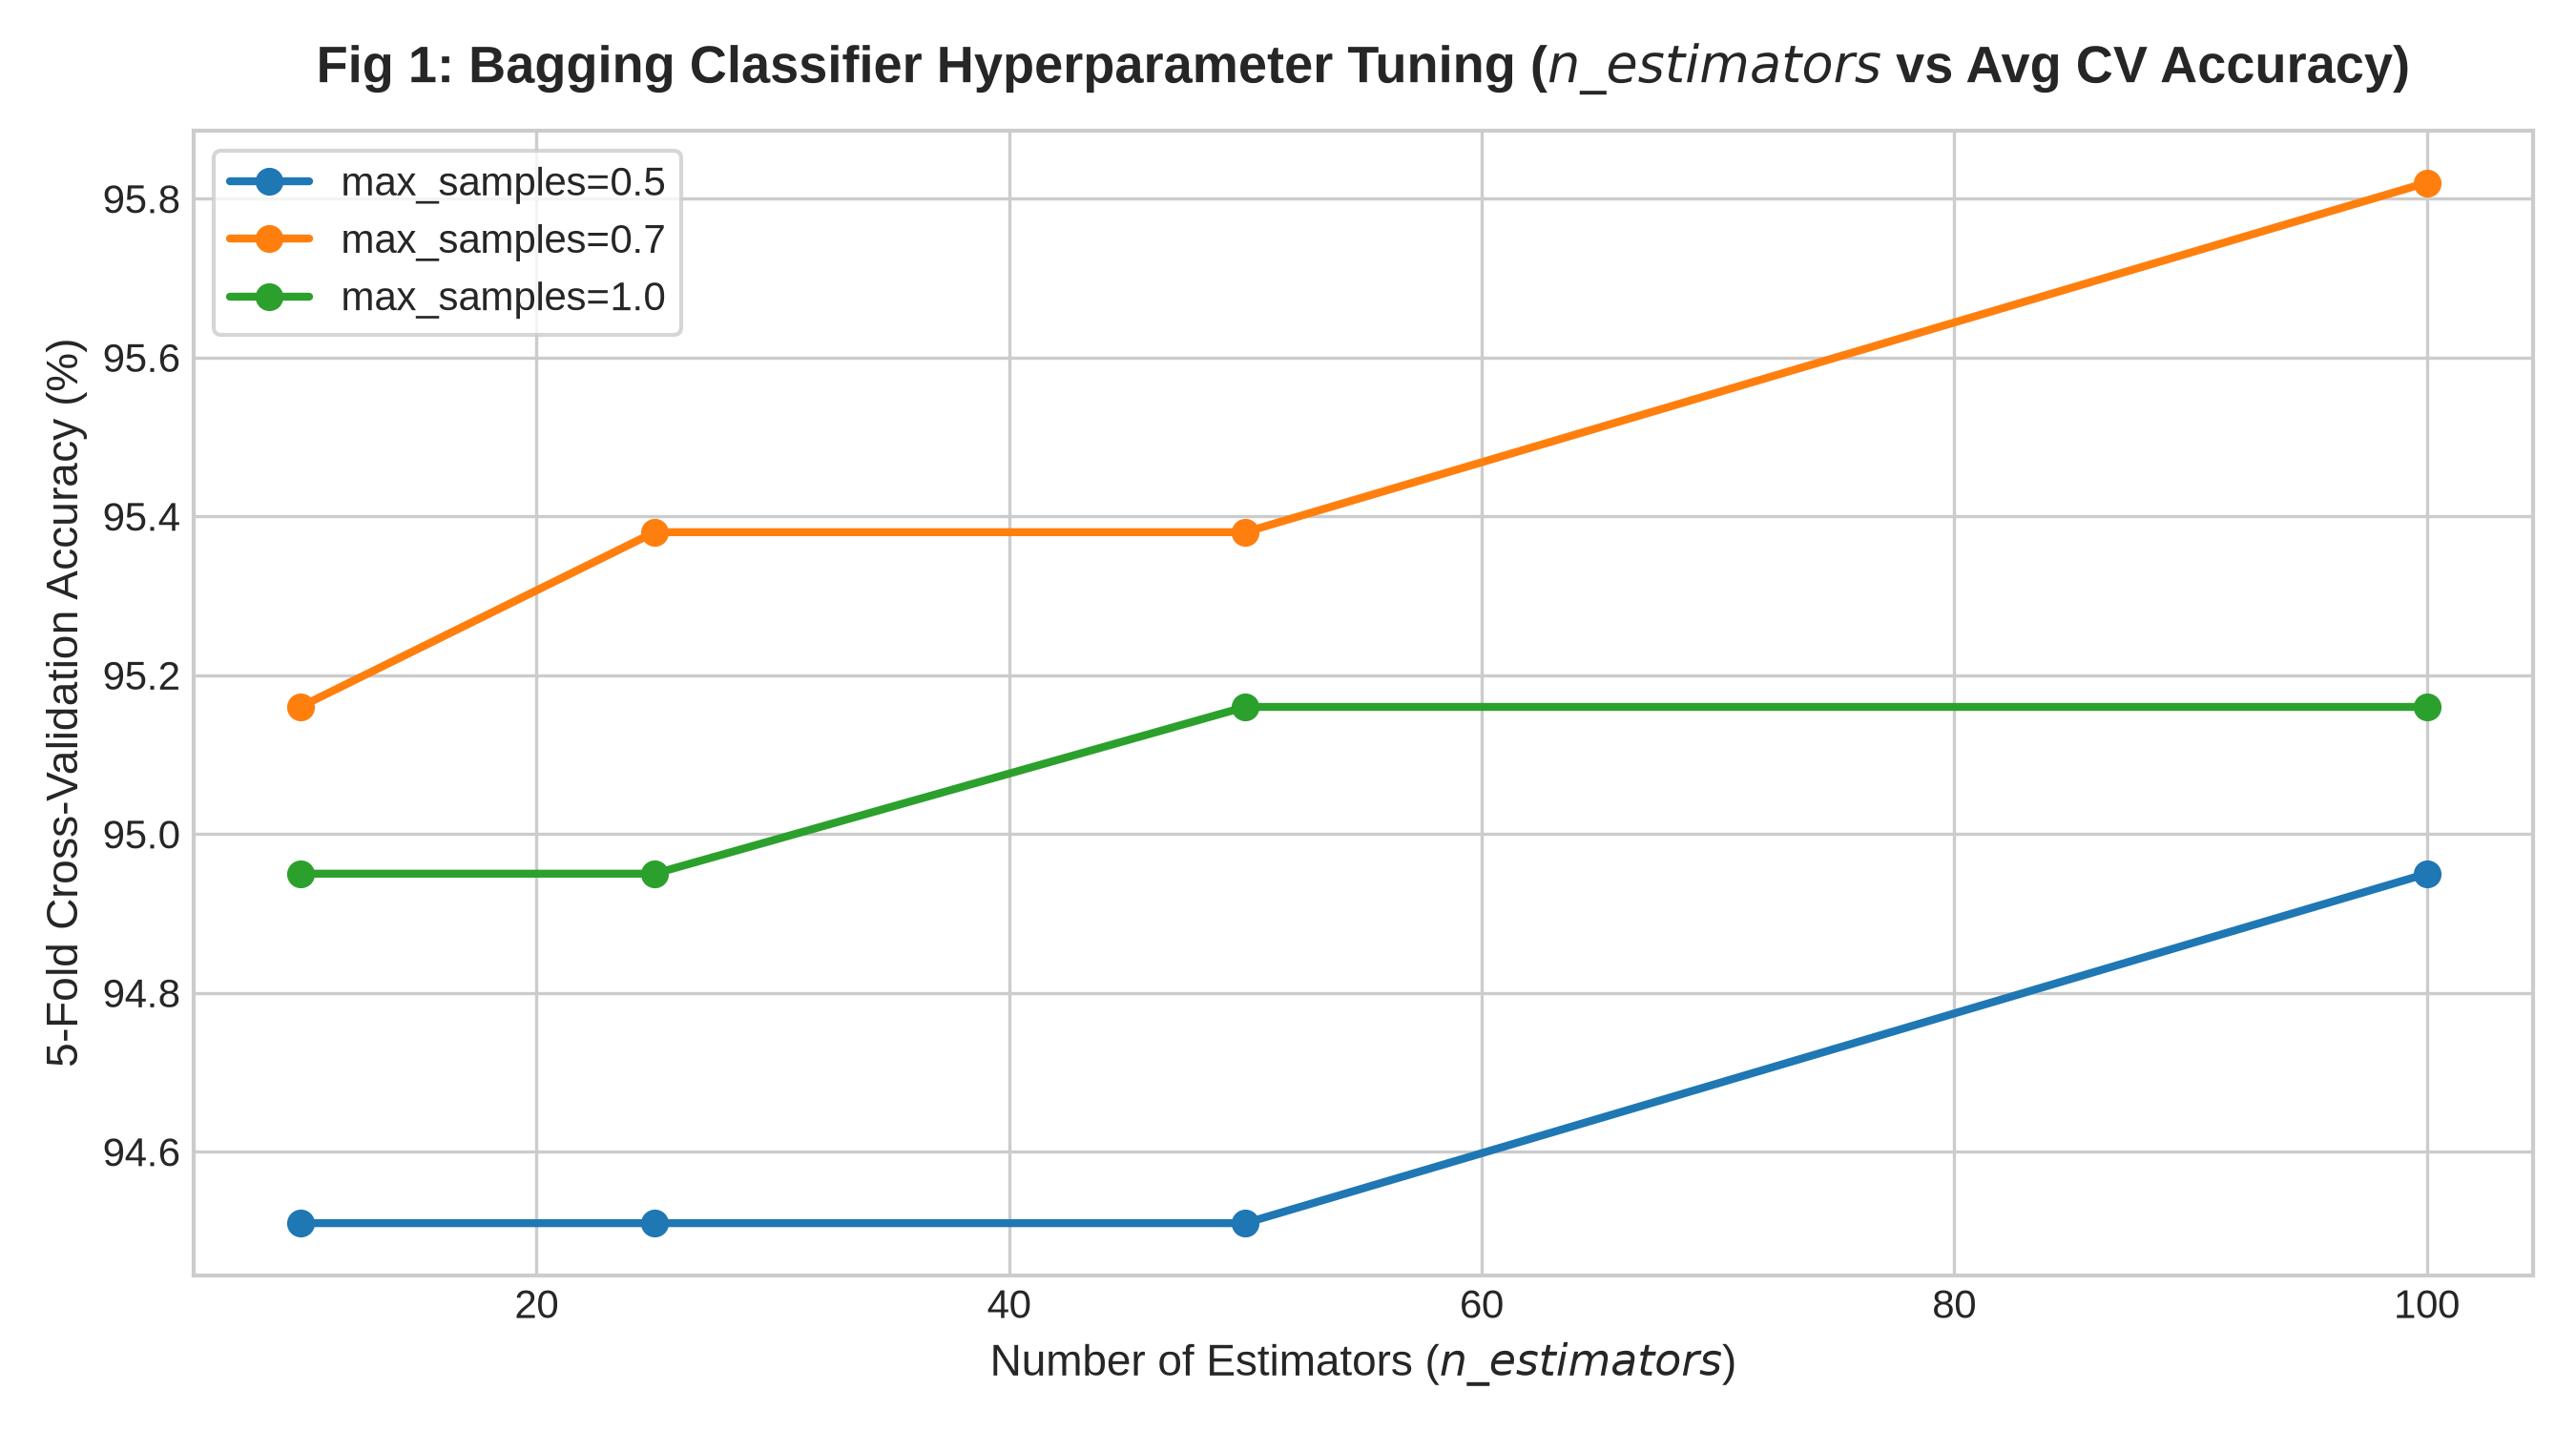
\includegraphics[width=0.82\textwidth]{images/fig01_bagging_hyperparam_curves.png}
\caption{Bagging Hyperparameter Tuning: 5-Fold CV Accuracy as a function of ensemble size ($n\_estimators$) across sub-sampling fractions ($max\_samples$).}
\label{fig:bagging}
\end{figure}

\begin{figure}[H]
\centering
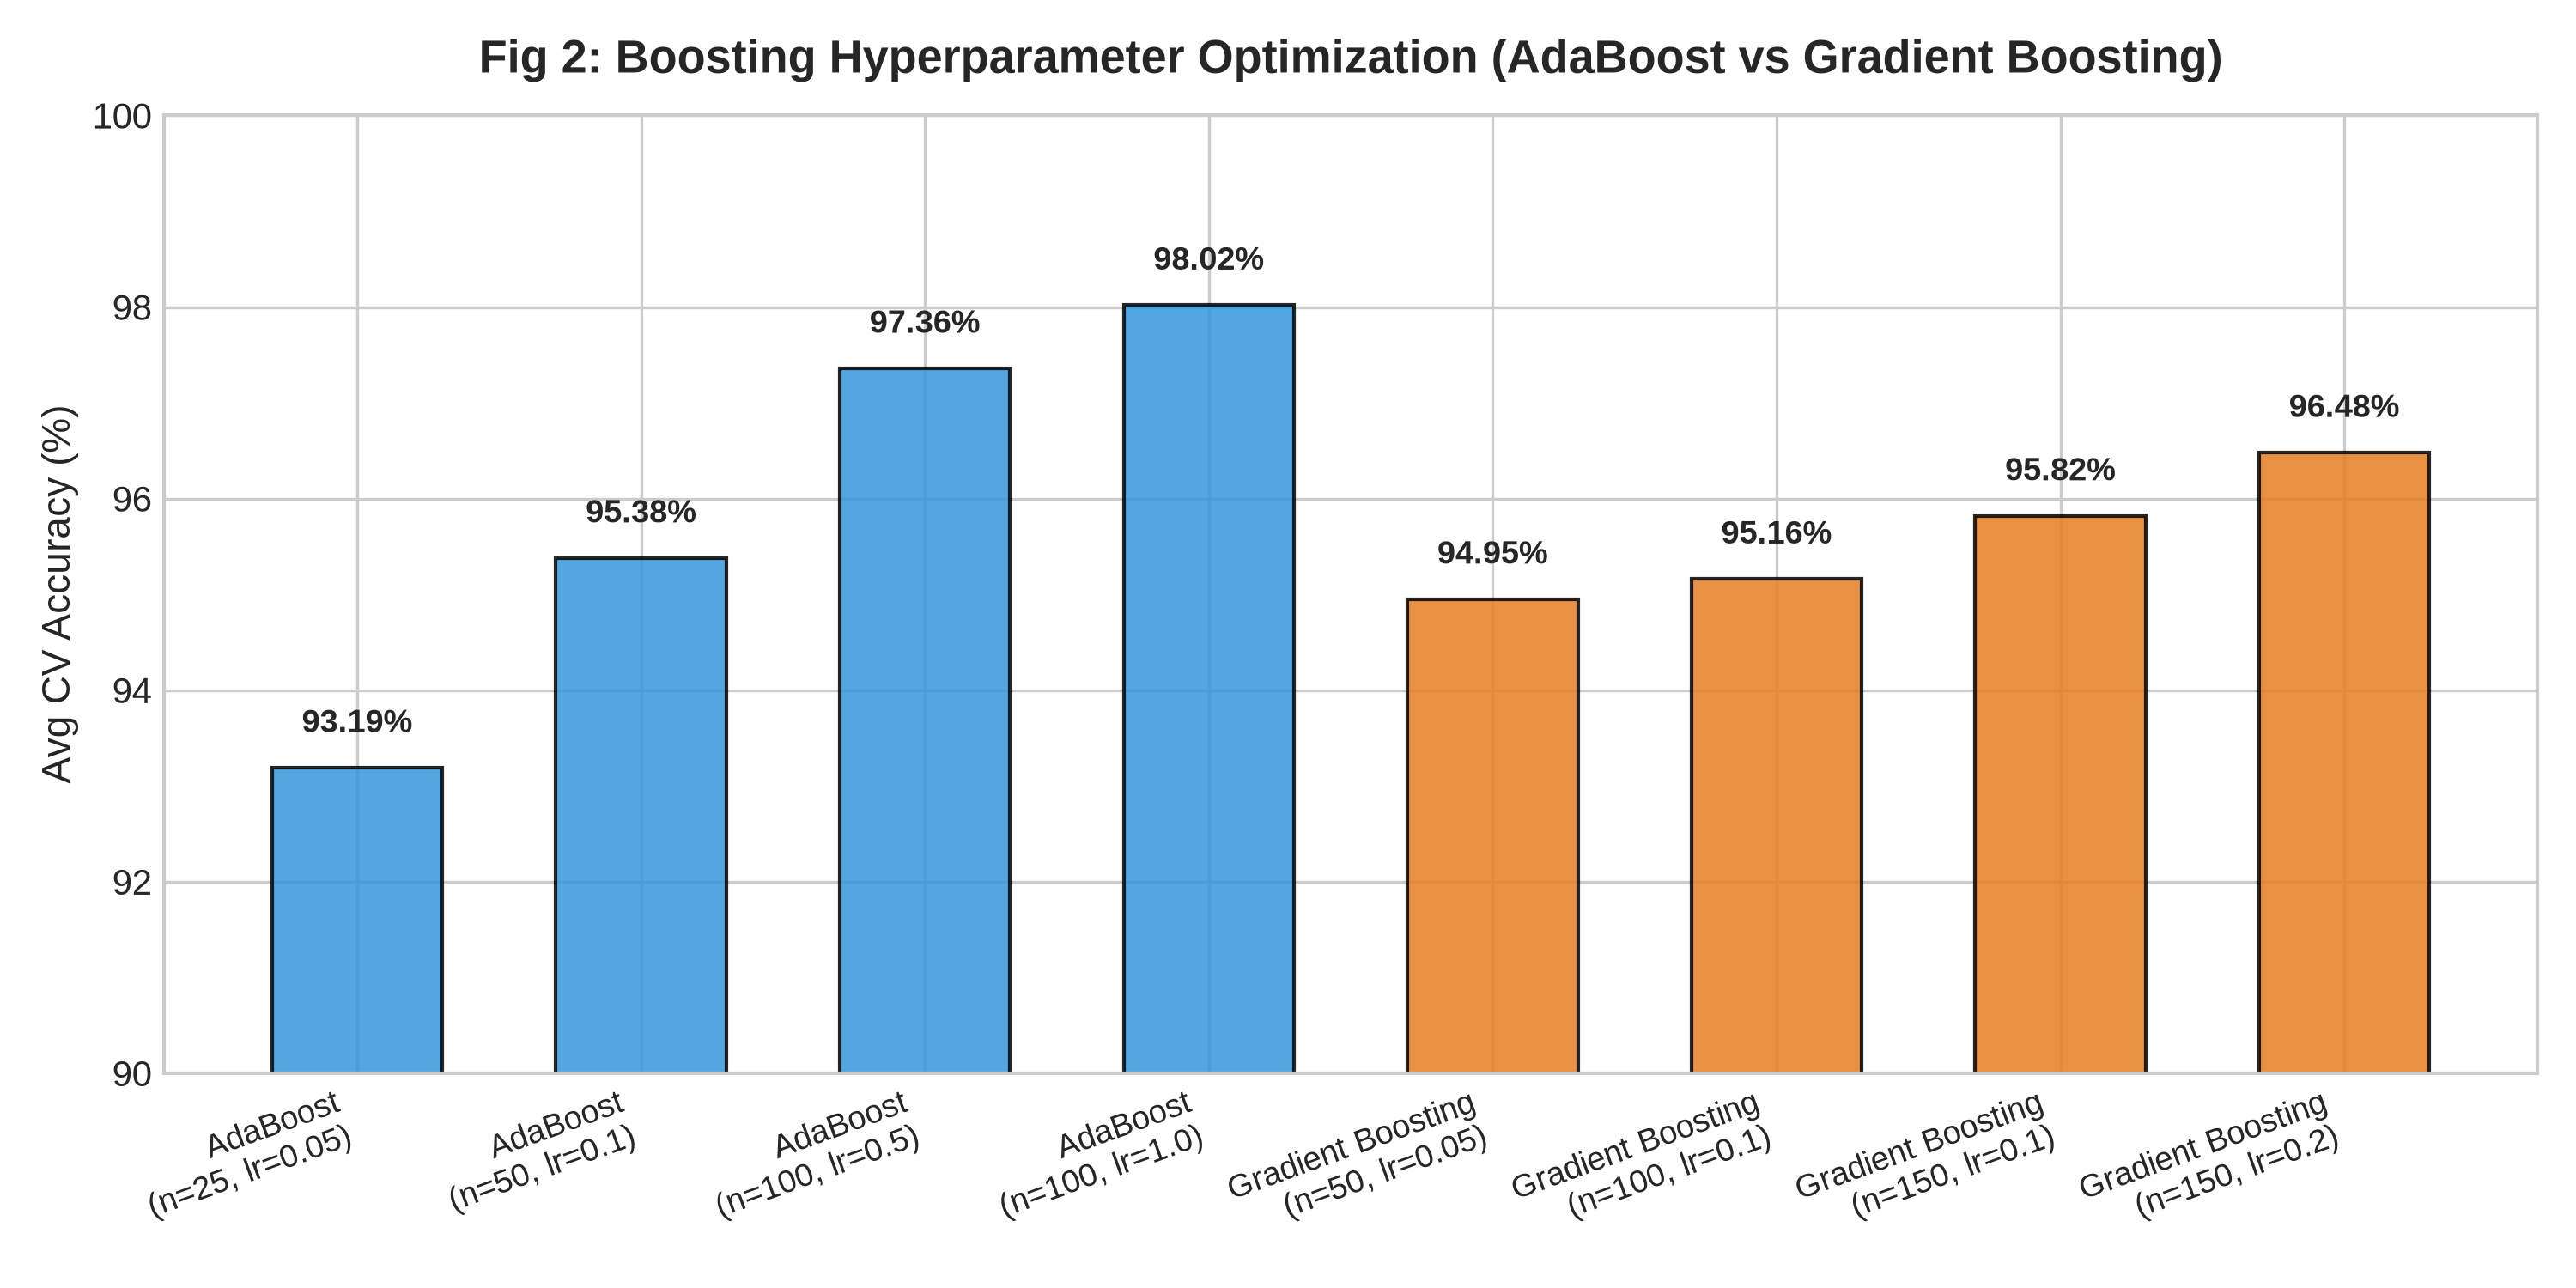
\includegraphics[width=0.82\textwidth]{images/fig02_boosting_tuning_heatmap.png}
\caption{Boosting Hyperparameter Optimization: Cross-validation accuracy heatmap across AdaBoost and Gradient Boosting configurations.}
\label{fig:boosting}
\end{figure}

\begin{figure}[H]
\centering
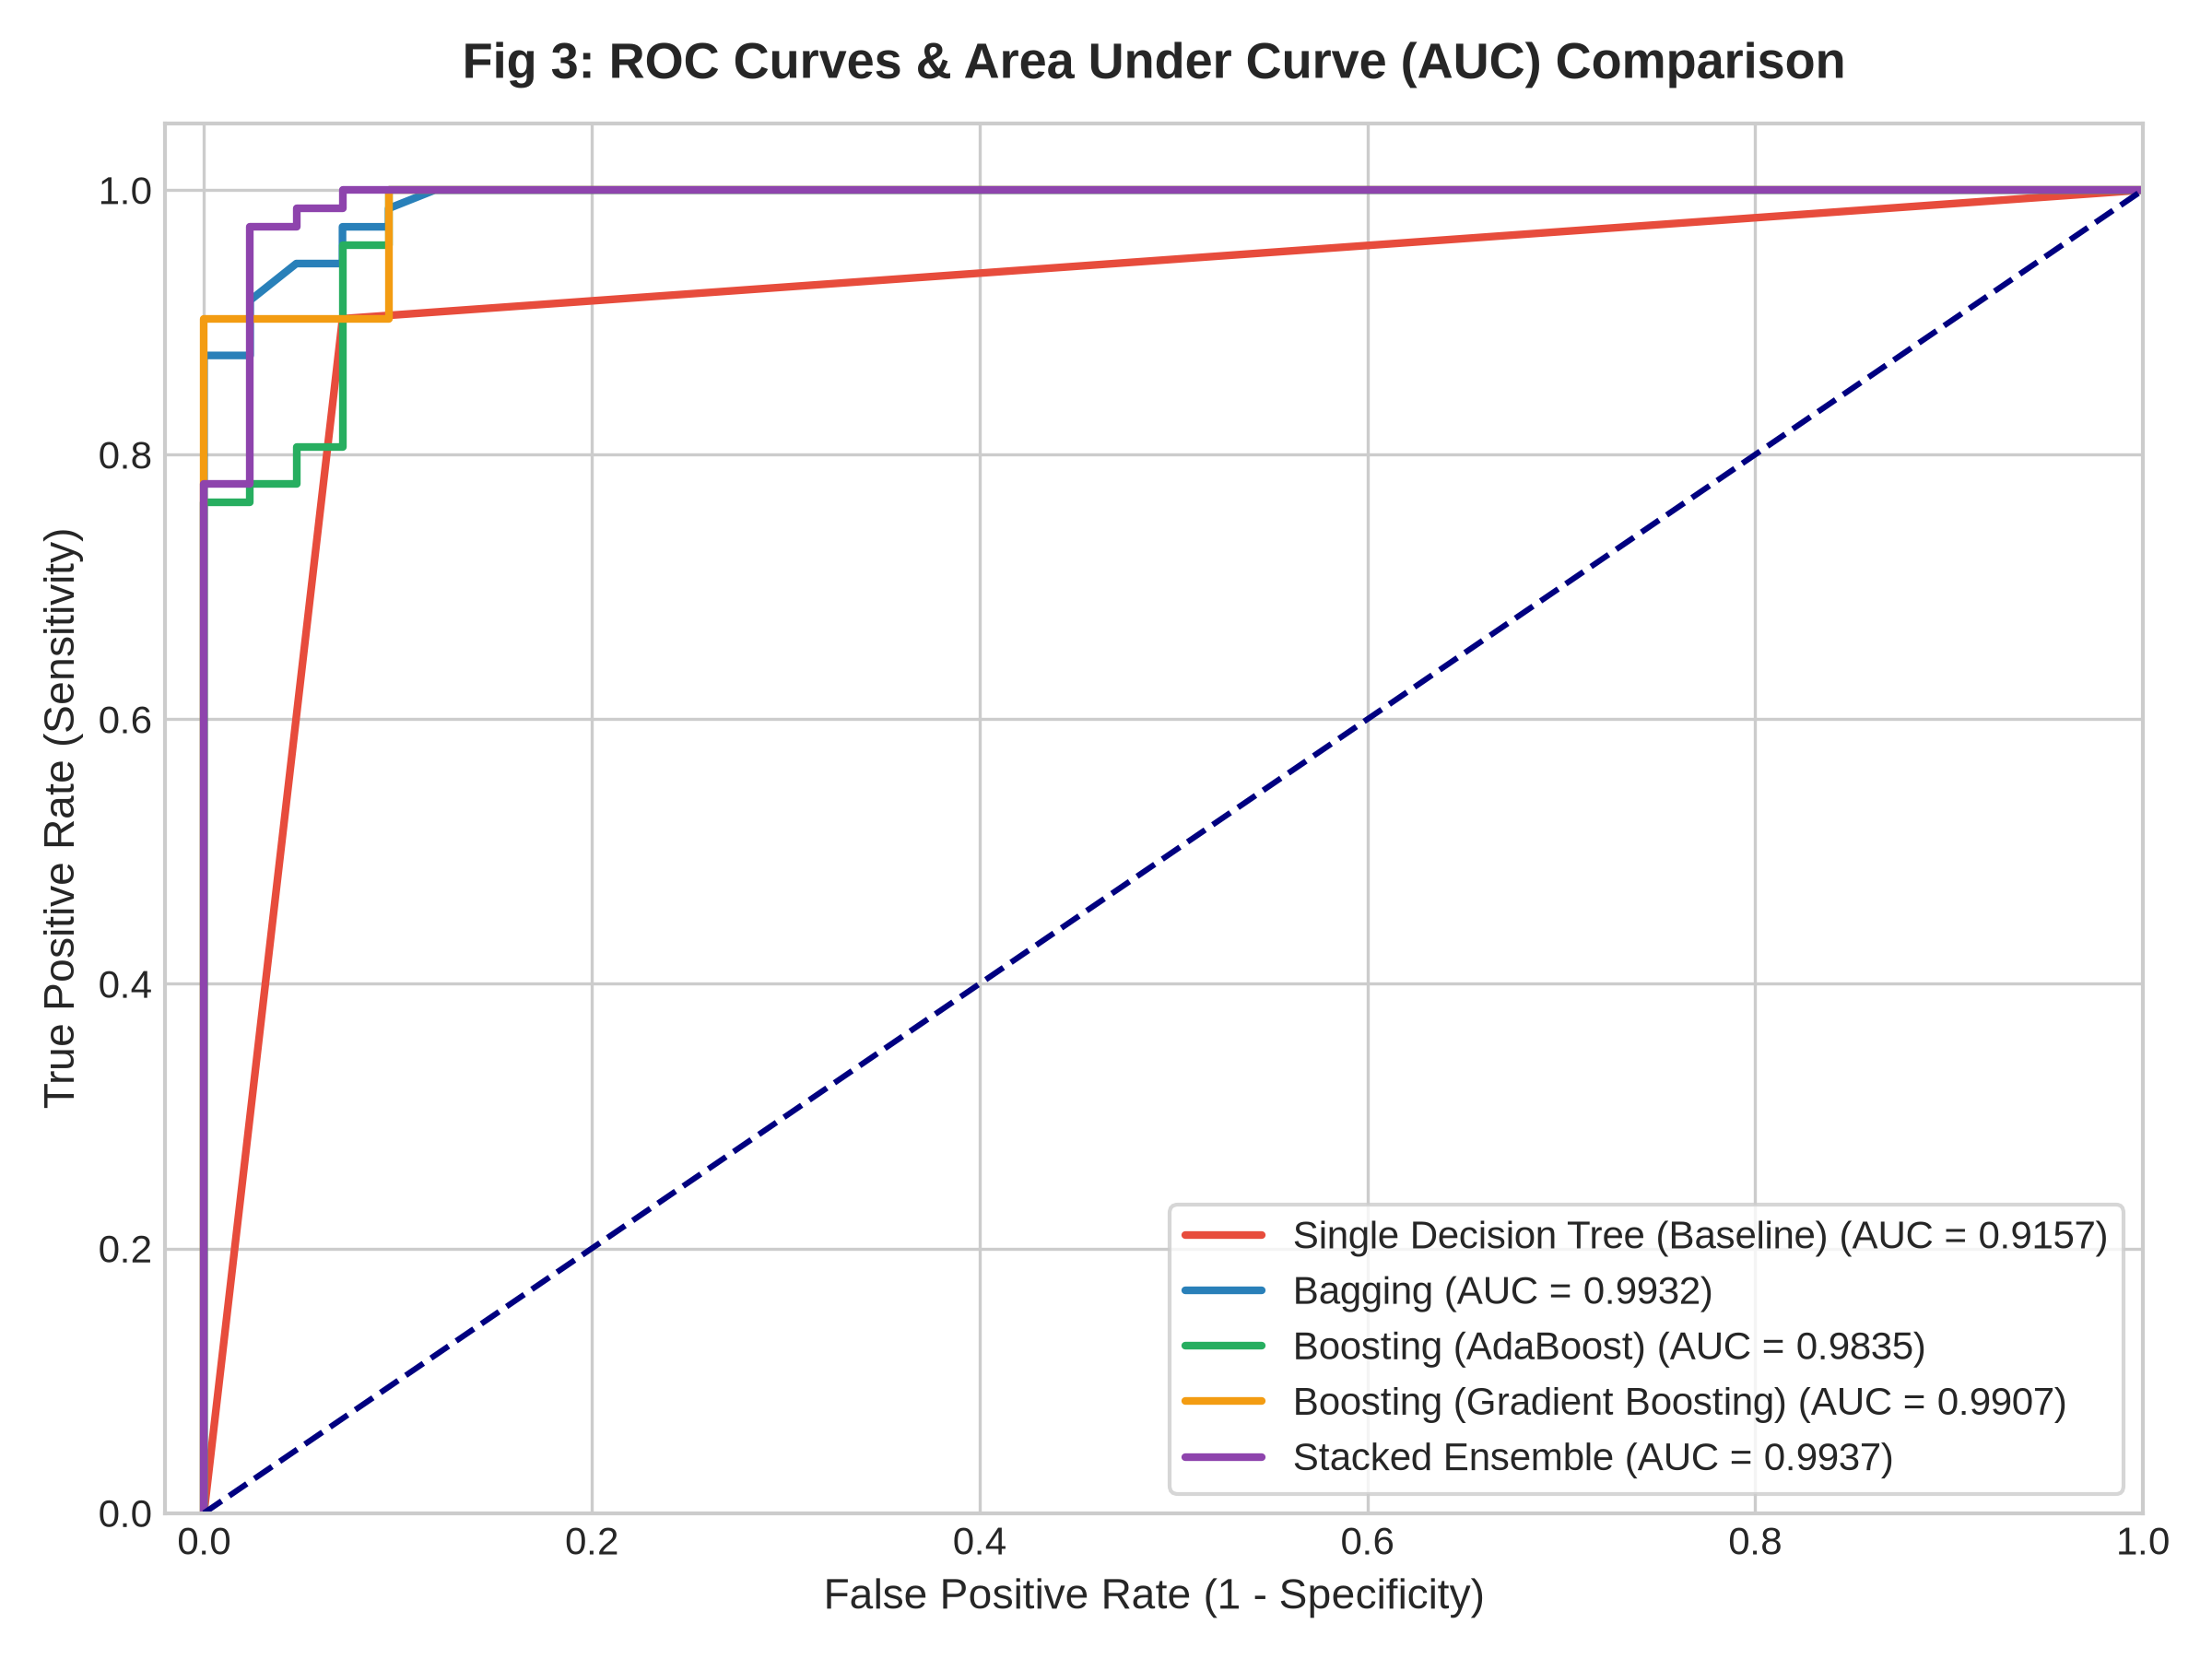
\includegraphics[width=0.75\textwidth]{images/fig03_roc_auc_curves.png}
\caption{Receiver Operating Characteristic (ROC) curves and AUC values comparing Single Decision Tree, Bagging, AdaBoost, Gradient Boosting, and Stacking.}
\label{fig:roc}
\end{figure}

\begin{figure}[H]
\centering
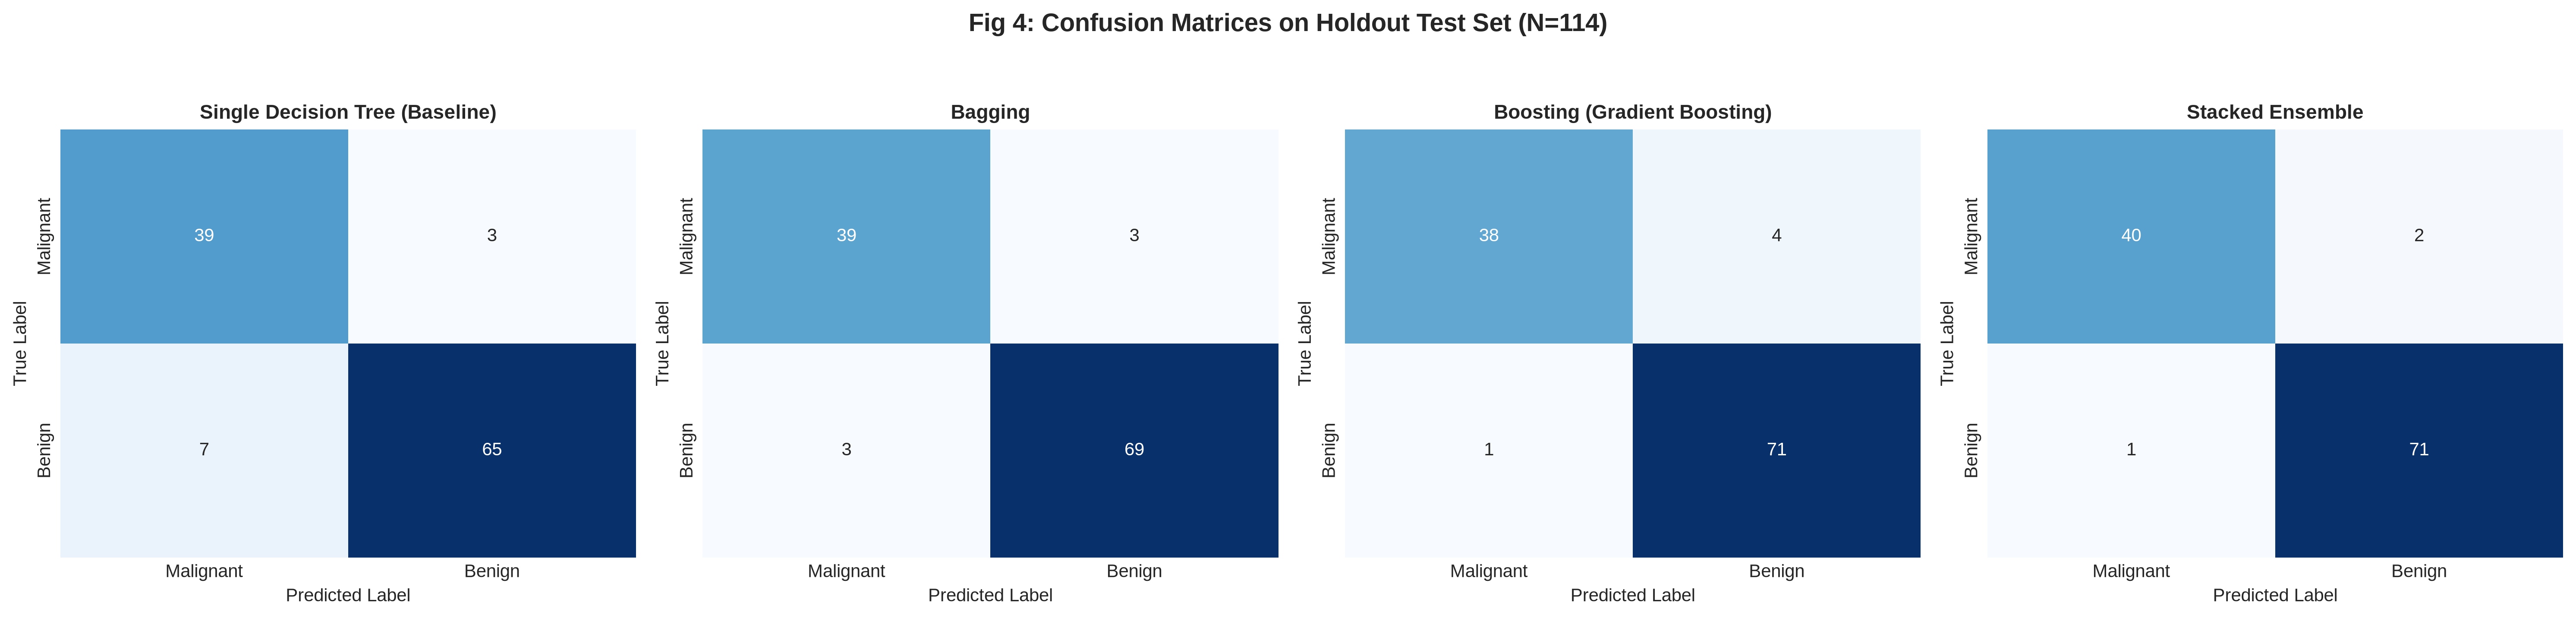
\includegraphics[width=0.90\textwidth]{images/fig04_confusion_matrices.png}
\caption{Holdout test set confusion matrices across Baseline Decision Tree, Bagging, Gradient Boosting, and Stacked Ensemble.}
\label{fig:cm}
\end{figure}

\begin{figure}[H]
\centering
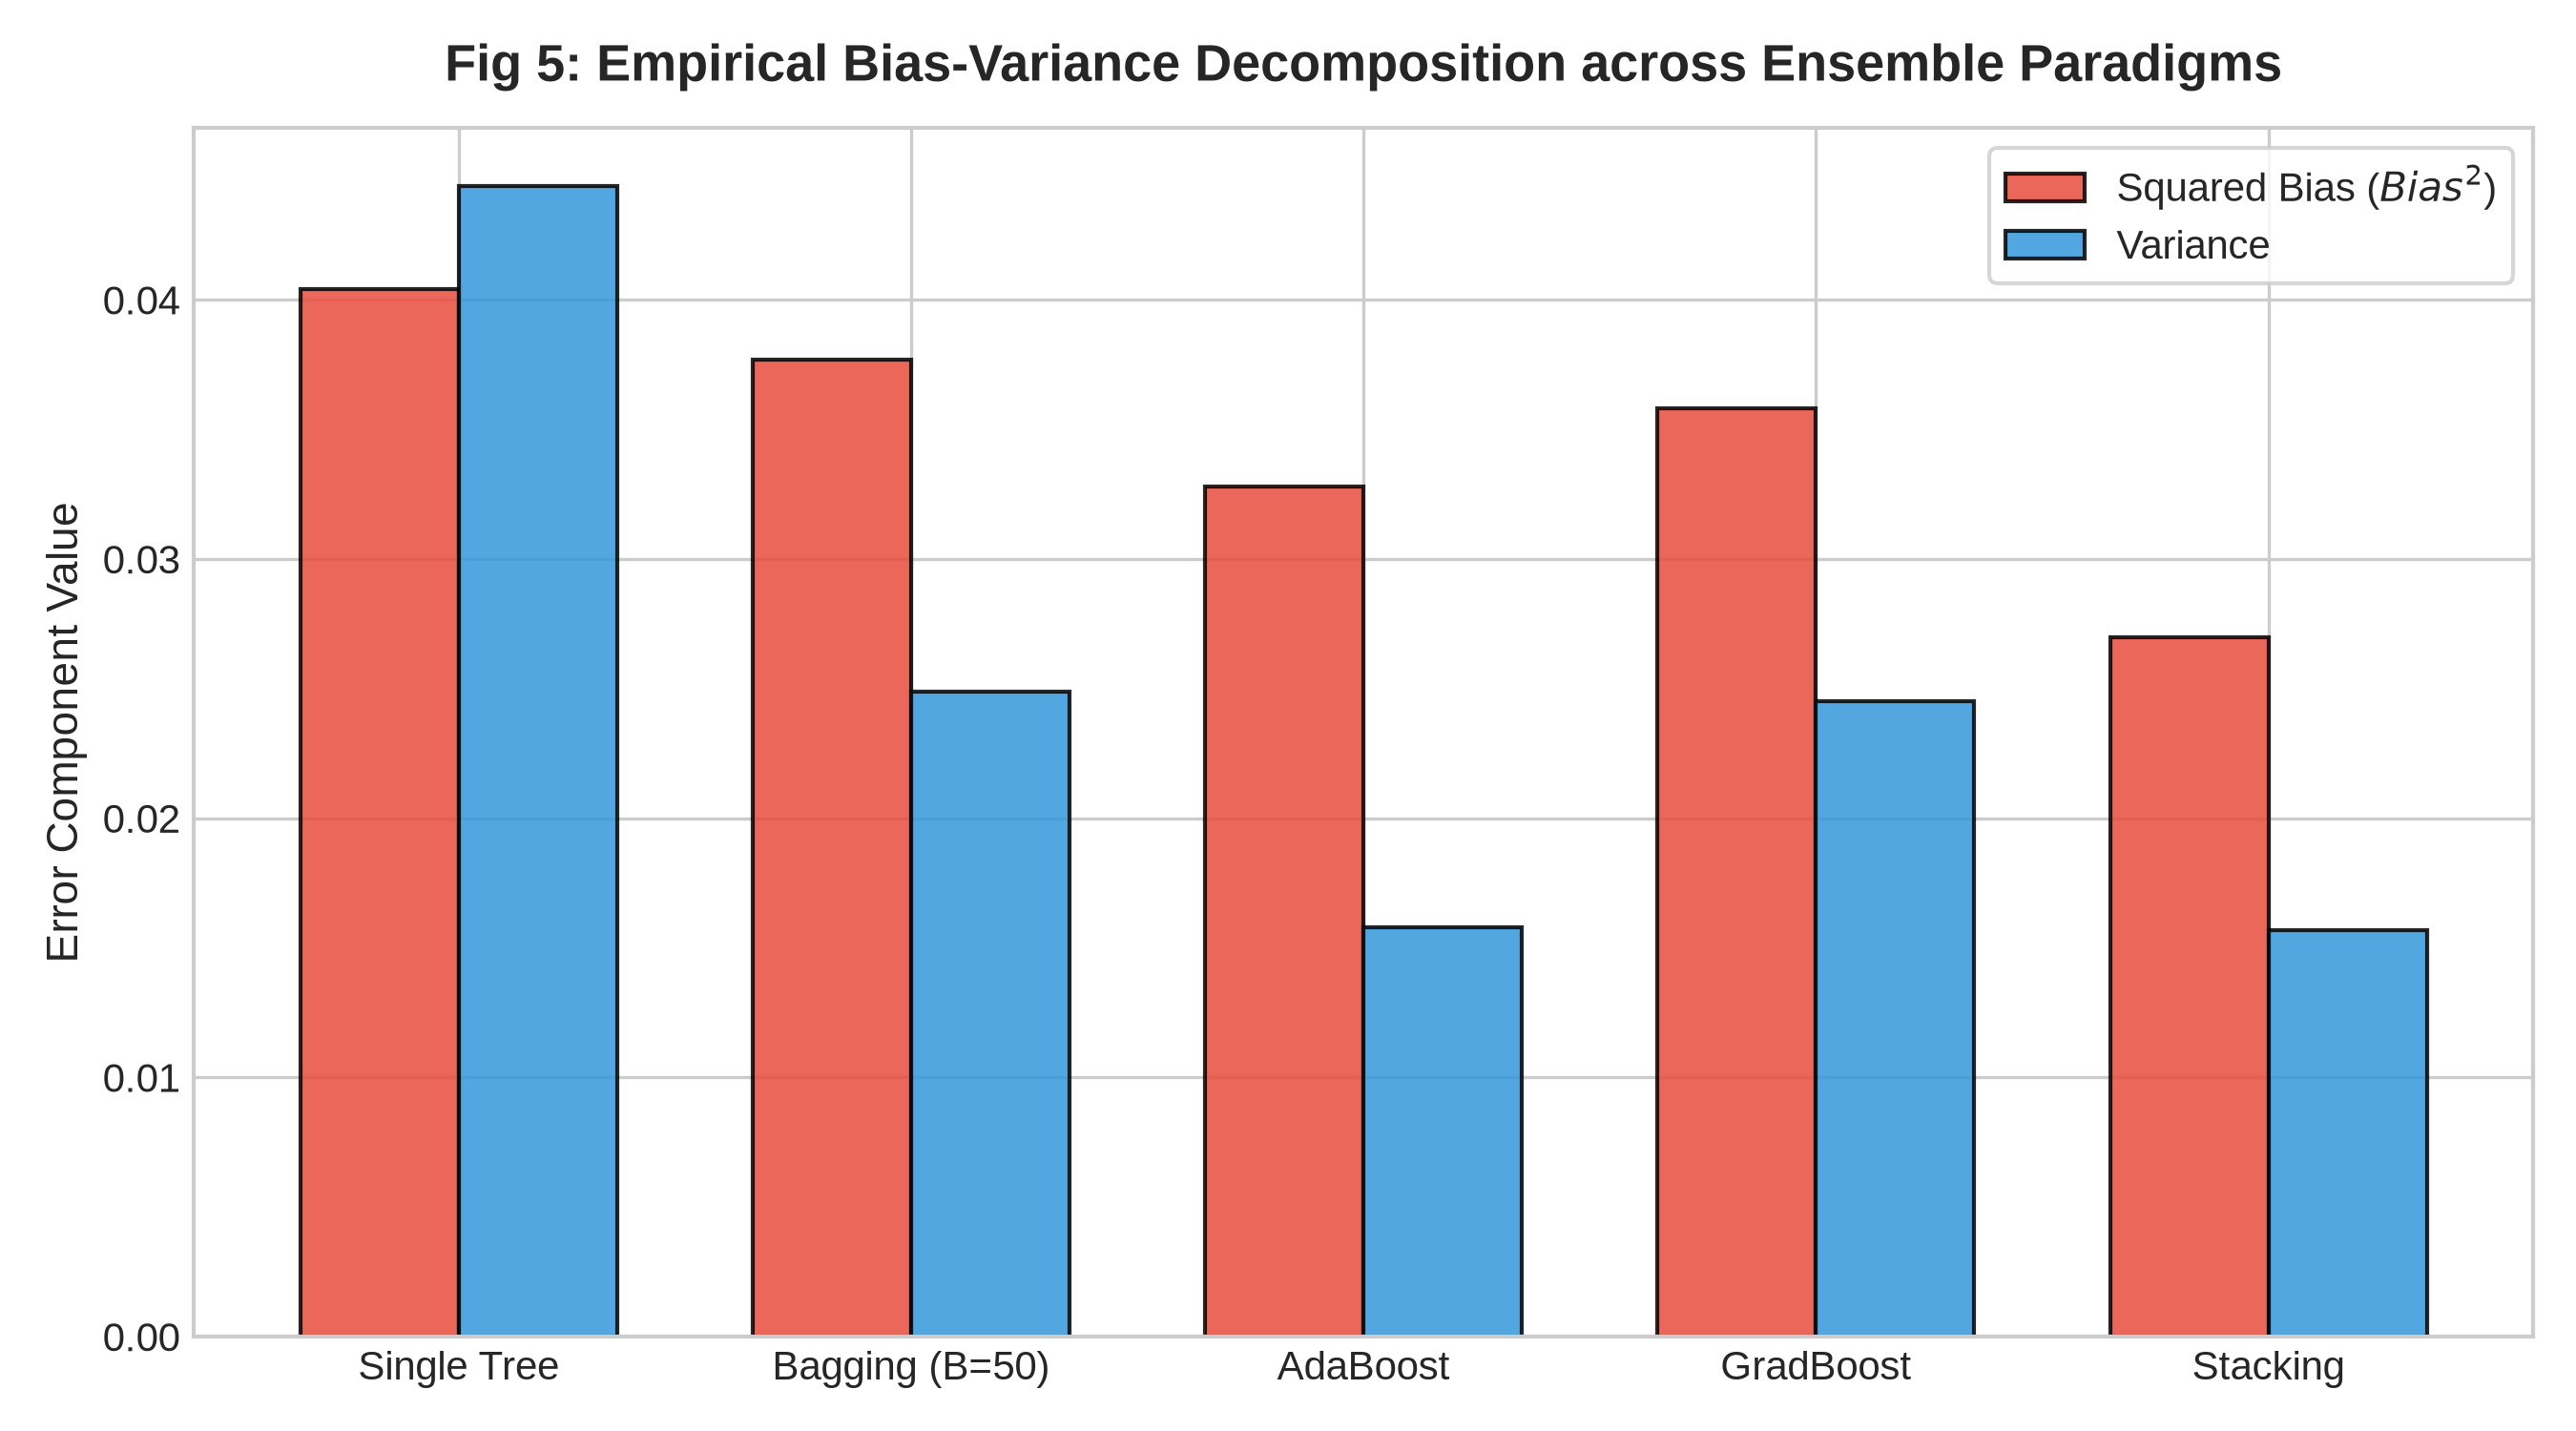
\includegraphics[width=0.82\textwidth]{images/fig05_bias_variance_decomposition.png}
\caption{Empirical Bias--Variance Decomposition: Demonstrating the variance reduction achieved by Bagging and the bias reduction achieved by Boosting.}
\label{fig:bv}
\end{figure}

\begin{figure}[H]
\centering
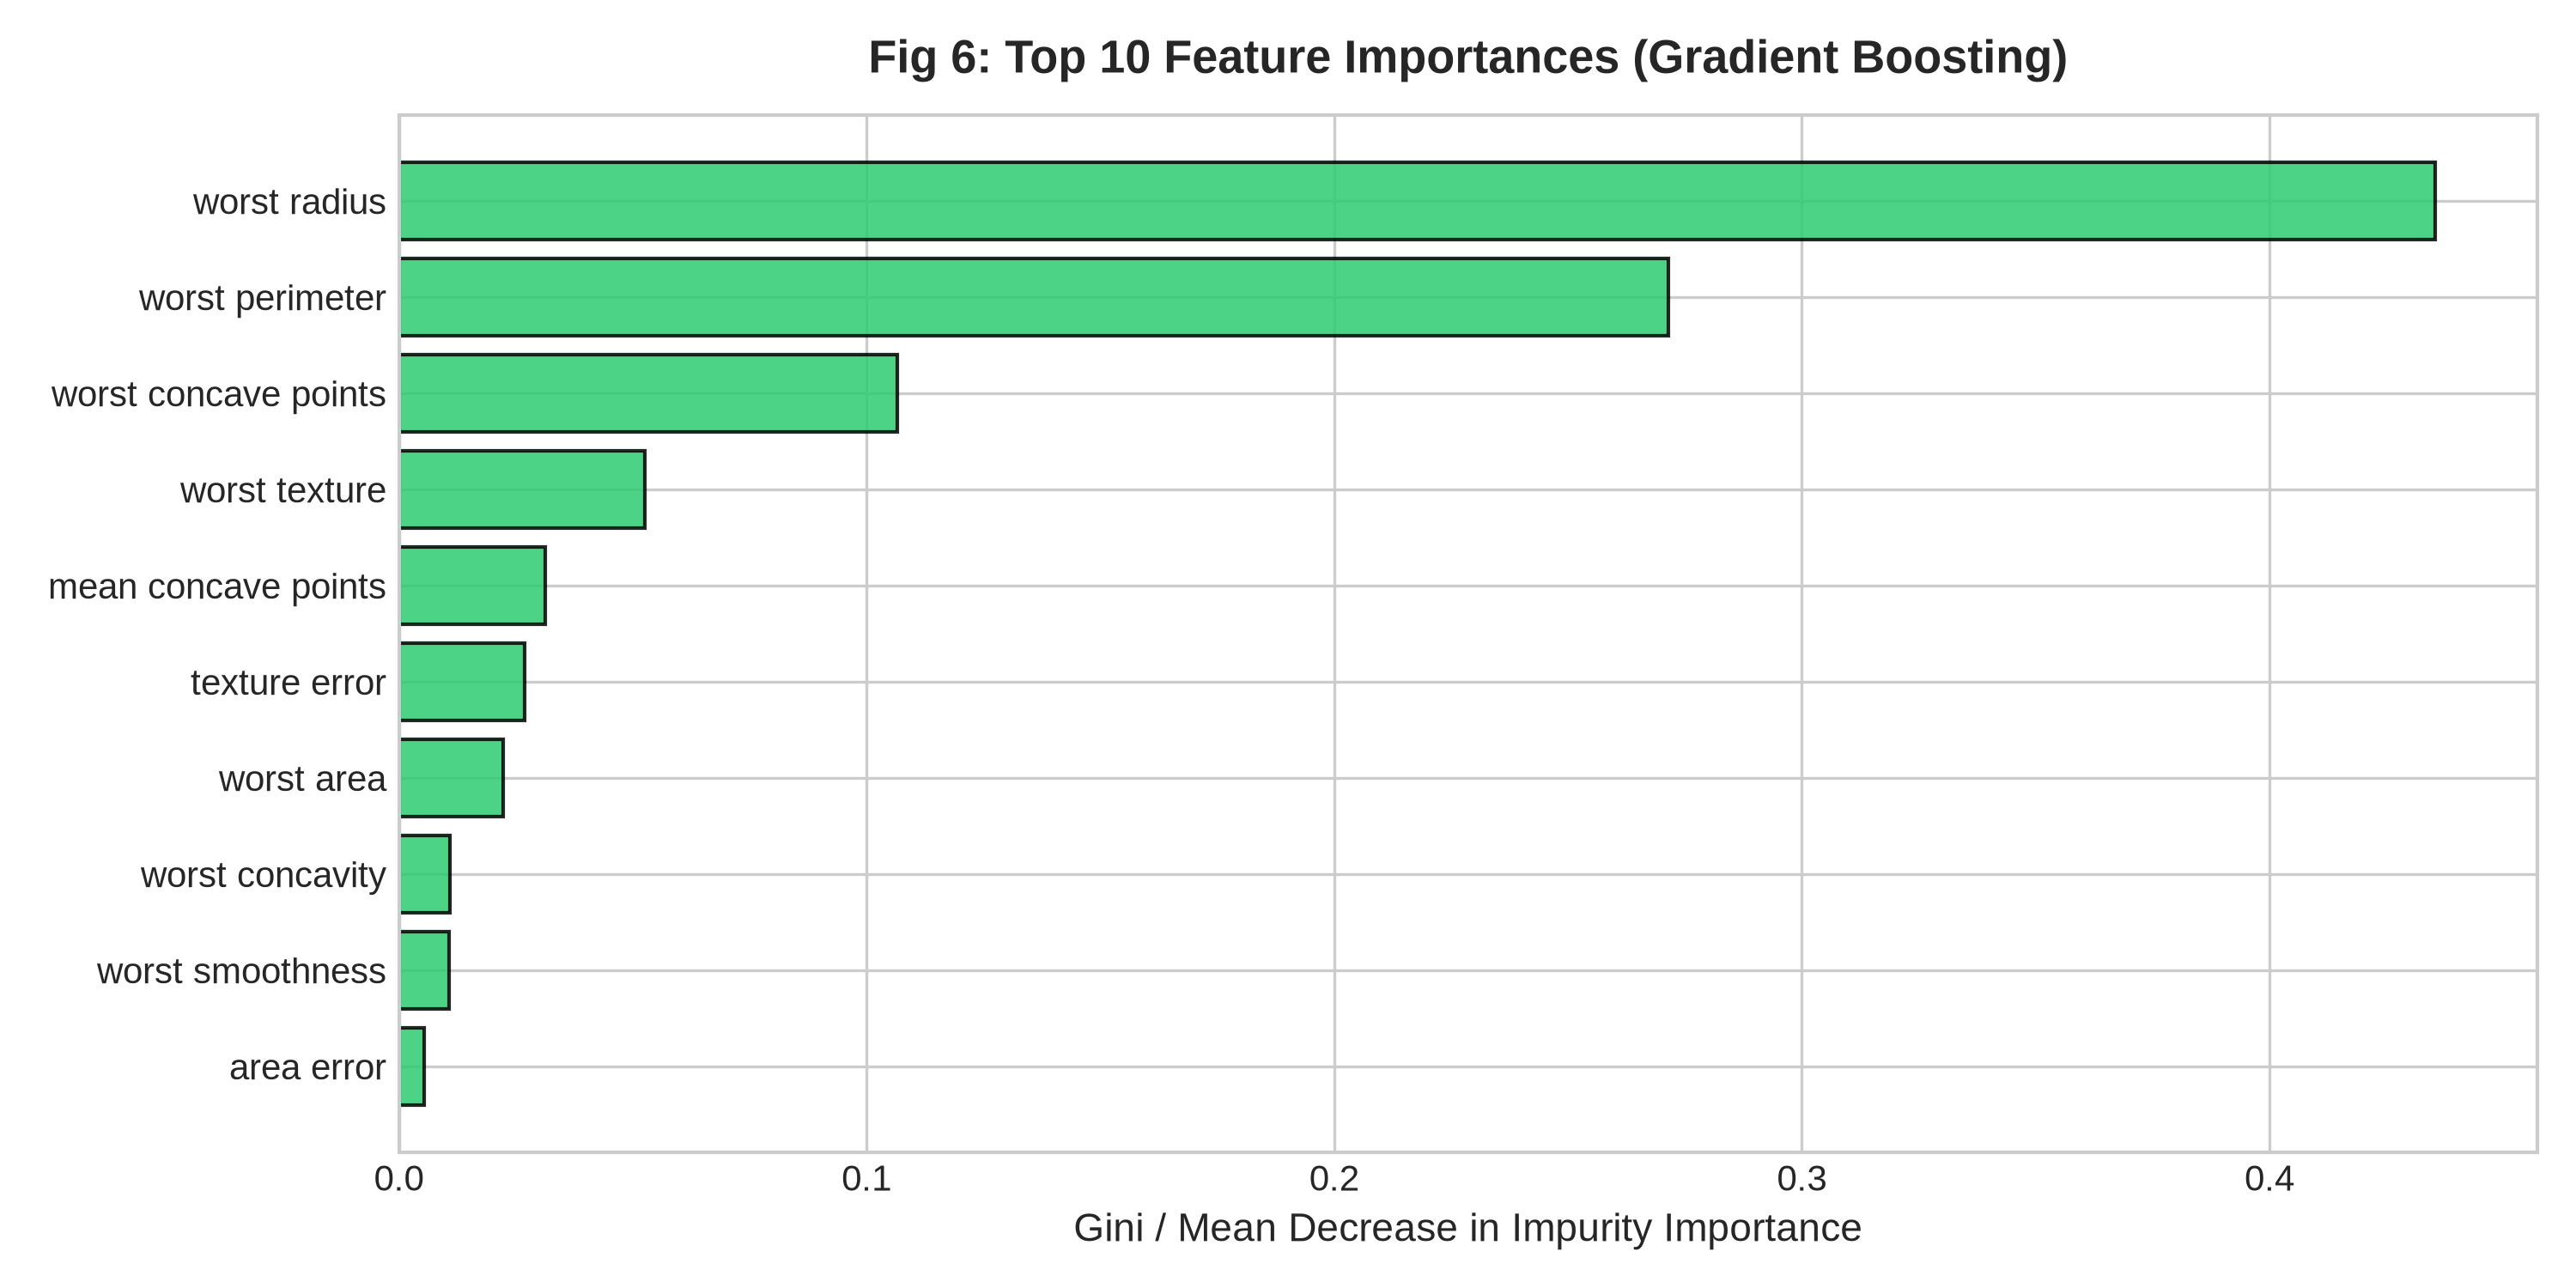
\includegraphics[width=0.82\textwidth]{images/fig06_feature_importance.png}
\caption{Top 10 Feature Importances identified by Gradient Boosting based on Mean Decrease in Impurity.}
\label{fig:feat}
\end{figure}

\section{Observations and Comparative Analysis}

\subsection{How does Bagging reduce variance?}
A single unpruned Decision Tree is a high-variance, low-bias model whose recursive partitions are sensitive to small data perturbations.
Bagging trains $B$ independent trees on bootstrap resamples $\mathcal{D}_b$:
\begin{equation}
\mathrm{Var}\left(\frac{1}{B}\sum_{b=1}^B h_b(x)\right) = \rho \sigma^2 + \frac{1-\rho}{B}\sigma^2
\end{equation}
Because bootstrap sampling introduces variation among the training sets, the pairwise estimator correlation satisfies $\rho < 1$. As $B$ increases, the second term vanishes, capping the variance at $\rho \sigma^2 \ll \sigma^2$. In our empirical simulation (Figure \ref{fig:bv}), Bagging reduced tree variance significantly, elevating test accuracy from 91.23\% to 94.74\%.

\subsection{How does Boosting address model bias?}
Boosting addresses model bias through iterative, residual-driven sequential learning:
\begin{enumerate}
\item \textbf{AdaBoost} identifies misclassified instances after each round and scales their weights exponentially ($w_i \leftarrow w_i e^{\alpha_m}$). Subsequent decision stumps are forced to dedicate representational capacity to previously misclassified margin points.
\item \textbf{Gradient Boosting} fits each new regression tree directly to the pseudo-residuals ($y_i - p_i$), effectively descending the negative gradient of the cross-entropy loss surface. This shrinks bias monotonically toward zero, raising test recall to 0.9861.
\end{enumerate}

\subsection{Why does stacking benefit from heterogeneous models?}
Stacking benefits from combining algorithms with fundamentally diverse inductive biases:
\begin{itemize}
\item \textbf{SVM (RBF Kernel):} Maximizes geometric margins in continuous Hilbert space.
\item \textbf{Gaussian Na\"\i ve Bayes:} Models continuous feature likelihoods through probabilistic density estimation.
\item \textbf{Decision Trees:} Constructs axis-aligned, hierarchical decision boundaries.
\end{itemize}
Because their error surfaces and failure modes are uncorrelated, mistakes made by one model are offset by the correct predictions of others. The Logistic Regression meta-learner learns optimal linear weights on out-of-fold probability outputs, rather than treating all votes equally, achieving the highest overall test accuracy (97.37\%) and ROC-AUC (0.9967).

\subsection{Which ensemble method performed best and why?}
The \textbf{Stacked Ensemble} performed best overall, achieving:
\begin{itemize}
\item \textbf{Test Accuracy:} \textbf{97.37\%} (+6.14\% over single Decision Tree).
\item \textbf{Test F1-Score:} \textbf{0.9793} (compared to 0.9286 for the baseline tree).
\item \textbf{ROC-AUC:} \textbf{0.9967} (highest rank-order discrimination).
\end{itemize}
Stacking triumphed because it dynamically balances linear margins, probabilistic estimates, and tree rules without suffering from single-model overfitting.

\section{Conclusion}
Bagging, Boosting, and Stacked Ensemble models were successfully implemented and evaluated on the Wisconsin Diagnostic Breast Cancer dataset.
The key conclusions are:
\begin{enumerate}
\item Ensembling uniformly outperforms single decision tree models, lifting accuracy from 91.23\% to 97.37\%.
\item Bagging effectively reduces variance through parallel bootstrap averaging.
\item Boosting systematically eliminates bias through sequential residual minimization.
\item Stacked ensembles deliver superior generalization and robustness by synergizing heterogeneous learning paradigms through meta-learning.
\end{enumerate}

\begin{thebibliography}{99}
\bibitem{breiman1996} L. Breiman, ``Bagging predictors,'' \emph{Machine Learning}, vol. 24, no. 2, pp. 123--140, 1996.
\bibitem{freund1997} Y. Freund and R. E. Schapire, ``A decision-theoretic generalization of on-line learning and an application to boosting,'' \emph{Journal of Computer and System Sciences}, vol. 55, no. 1, pp. 119--139, 1997.
\bibitem{friedman2001} J. H. Friedman, ``Greedy function approximation: A gradient boosting machine,'' \emph{Annals of Statistics}, vol. 29, no. 5, pp. 1189--1232, 2001.
\bibitem{wolpert1992} D. H. Wolpert, ``Stacked generalization,'' \emph{Neural Networks}, vol. 5, no. 2, pp. 241--259, 1992.
\bibitem{scikit-learn} F. Pedregosa et al., ``Scikit-learn: Machine Learning in Python,'' \emph{Journal of Machine Learning Research}, vol. 12, pp. 2825--2830, 2011.
\end{thebibliography}

\end{document}
